% =====================================================================
%  Submission to AID 2026 -- 2nd IEEE PRDC Workshop on AI Dependability
%  DOUBLE-BLIND: no author, no affiliation, no e-mail, no repository URL.
%  Hard limit: 6 pages including figures, tables and references.
%  Body follows the author's original draft (adv-multimodal-llm.tex),
%  condensed to the page limit and updated with the new measurements
%  recorded in NUMBERS.md.  See EXTENDED-NOTES.md for what was cut.
% =====================================================================
\documentclass[conference]{IEEEtran}
\IEEEoverridecommandlockouts

\usepackage[utf8]{inputenc}
\usepackage[T1]{fontenc}
\usepackage{amsmath}
\usepackage{amsfonts}
\usepackage{amssymb}
\usepackage{graphicx}
\usepackage{booktabs}
\usepackage{multirow}
\usepackage{xcolor}
\usepackage{microtype}
\usepackage{tikz}
\usepackage{pgfplots}
\pgfplotsset{compat=1.18}
\usepackage{url}
\usetikzlibrary{positioning,calc}
\usepackage[hidelinks]{hyperref}
\usepackage[capitalise,nameinlink]{cleveref}

% ---- strip identifying PDF metadata (double-blind) ----
\hypersetup{
  pdfauthor={},
  pdfsubject={},
  pdfkeywords={},
  pdfcreator={},
  pdfproducer={},
  pdftitle={Anonymous submission}
}

\crefname{figure}{Fig.}{Figs.}
\Crefname{figure}{Fig.}{Figs.}
\crefname{table}{Table}{Tables}
\Crefname{table}{Table}{Tables}
\crefname{section}{Sec.}{Secs.}
\Crefname{section}{Sec.}{Secs.}

% two-value cell: gray = accuracy on ground-truth label, black = targeted success
\newcommand{\cell}[2]{{\color{gray}#1}\,/\,#2}
\newcommand{\ccell}[1]{{\color{gray}#1}}

% prompt-mode illustration: highlight colors
\definecolor{hlQ}{HTML}{D6E4F0} % question / prompt
\definecolor{hlP}{HTML}{FCE5CD} % answer priming
\definecolor{hlT}{HTML}{D9EAD3} % teacher-forced candidate
\definecolor{barcol}{HTML}{3D6FB4}
\newcommand{\hlQ}[1]{\colorbox{hlQ}{#1}}
\newcommand{\hlP}[1]{\colorbox{hlP}{#1}}
\newcommand{\hlT}[1]{\colorbox{hlT}{#1}}
\newcommand{\logit}[1]{\textcolor{barcol}{\rule[-0.3ex]{#1pt}{1.3ex}}}

% compact quote environment for verbatim model Q&A
% (replaces the `framed'-based qatext, which breaks in a narrow column)
\newenvironment{qa}%
  {\par\addvspace{2pt}\begingroup\footnotesize
   \setlength{\leftskip}{0.9em}\setlength{\parindent}{0pt}\setlength{\parskip}{1pt}}%
  {\par\endgroup\addvspace{2pt}}

% ---- helper macros (the in-flight placeholders they served are all resolved) ----
\newcommand{\PH}[1]{\textcolor{gray}{\textit{#1}}}

% IEEEtran typesets TABLE captions in \scshape (IEEEtran.cls, \@makecaption
% branches at L2737/L2778); figure captions are unaffected. That suits a
% three-word caption but turns a multi-sentence one into a wall of small caps.
% \tabcap restores normal text for table captions only, without patching the
% class: the leading \normalfont overrides the \scshape the class just applied.
\newcommand{\tabcap}[1]{\caption{\normalfont #1}}
\newcommand{\reserve}[2]{% #1 = reserved height, #2 = label
  \setlength{\fboxsep}{2pt}%
  \fbox{\parbox[c][#1][c]{\dimexpr\linewidth-2\fboxsep-2\fboxrule\relax}%
        {\centering\scriptsize\color{gray}#2\par}}}

\title{Shared Encoder, Unshared Safety:\\
Adversarial Images across CLIP-Based VLMs}

% Double-blind: authors, affiliations and contact details withheld.
\author{\IEEEauthorblockN{Anonymous Submission}}

\begin{document}
\maketitle

\begin{abstract}
Adversarial examples expose the vulnerability of image classifiers and
visual encoders. As language models acquire visual modalities (VLMs), it
matters whether they inherit that vulnerability, and how far adversarial
examples transfer among VLMs sharing one encoder. Our experiments use CLIP
and two VLMs built on it, LLaVA and VisualRWKV, with image classification
on Imagenette. Our result shows that adversarial examples trained on
visual encoders are more transferable, and that end-to-end adversarial
training overfits on the language model and the target prompt. For harmful
requests, we discover universal adversarial images that raise the
compliance rate on the PKU-SafeRLHF dataset, but neither image transfers to
the other VLM: the shared encoder carries the classification attack, not
the jailbreak. We also find that neither instrument is stable: the attack
succeeds in about half of identically configured attempts, and four LLM
judges score the same generations from $6\%$ to $85\%$. Cheap input
transformations blunt both attacks, except bit-depth reduction, which stops
only the first.
\end{abstract}

\begin{IEEEkeywords}
adversarial examples, vision--language models, transferability, safety
alignment, dependability
\end{IEEEkeywords}

\section{Introduction}

Machine learning models now have human-level capabilities in many tasks,
but they follow a totally different mechanism from humans and have unique
vulnerabilities. Adversarial example is such a case. It refers to
the scenario that attackers can construct input examples that steer and
change the output in an unexpected way. One typical type of adversarial
examples happens in image classification: Szegedy et
al.~\cite{Szegedy2014Intriguing} showed that an imperceptible perturbation
obtained by box-constrained optimization is enough to make a
state-of-the-art classifier assign an arbitrary wrong label with high
confidence. The adversarial examples are not distinguishable with clean
ones to human eyes, and this discovery reveals a type of real and critical
vulnerability that can be utilized maliciously.

Adversarial example follows the form of a white-box attack. The attacker
has knowledge of the entire inference structure and weight of the model.
The adversarial example is fabricated by minimizing the cross-entropy loss
on the target label, and performing gradient descent on the input example
rather than model weight. The common explanation for the existence of
adversarial examples is the large input space: for images with 8 bit-depth
and 3 channels, the total count of all possible variants goes to
$256^{3\times W \times H}$ for an image of $W\times H$ pixels. It is
therefore easy to find approximate but
out-of-distribution samples that the model has never seen, and adversarial
examples exploit this fact.

With the surge of LLM in recent years, it would be meaningful to ask
whether similar attacks can be performed on language models, especially
those with multiple modalities besides text. The design of multimodal
language models usually consists of one pretrained language model backbone,
and the encoders that embed multimodal input as tokens in the LM semantic
space. Therefore, it would be likely that multimodal language models
inherit the vulnerability of encoders as well. And since language models
process and generate text, there are even more aspects exposed to
adversarial example attacks other than simple classification. For example,
an attacker may be able to bypass the safeguard or retrieve sensitive
information with an adversarial image input. Another concern is the
transferability of adversarial examples. Since different models may share
the same encoder, we want to understand how generic the adversarial
examples are -- what a shared encoder does, and does not, make portable.

This work focuses on Visual Language Models based on the CLIP visual
encoder, and studies the construction and transferability of adversarial
examples. In particular, we choose two VLMs that use CLIP as the visual
encoder: LLaVA-1.5 7B~\cite{Liu2024LLaVA15} and VisualRWKV-6
7B~\cite{Hou2025VisualRWKV}. We investigate attacks on image classification
and jailbreaks. Our results show that these VLMs are vulnerable to
adversarial image attacks, and the examples are transferable in general. In
classification, we find that adversarial examples trained only on the
visual encoder work in more general cases than those trained end-to-end on
LLaVA, over the whole range of perturbation budgets we swept. These
discoveries suggest
that the vulnerability does come from the encoder, and the end-to-end
training of adversarial examples will overfit on the language model
backbone. For adversarial examples causing jailbreaks, we discover
universal adversarial images that substantially increase the compliance
rate of both VLMs on harmful requests from the PKU-SafeRLHF dataset. Unlike
the classification attack on the encoder, these jailbreaks do not transfer
between the two VLMs in either direction despite the shared encoder, which
suggests that the safeguard ability lies mainly in the language model
backbone. A third result concerns the experiment rather than the models: the jailbreak
attack is not repeatable. Identically configured runs succeed about half the
time, fixing the seed does not help, and four LLM judges score one identical
set of generations from $6\%$ to $85\%$.
Finally, we test four cheap input transformations as defenses, and find that
they blunt both attacks -- with one instructive exception.
Code will be released upon publication.

\section{Related Work}

The first adversarial example attack was proposed by Szegedy et
al.~\cite{Szegedy2014Intriguing}. They reported that imperceptible
perturbation obtained by box-constrained optimization can mislead image
classifiers.

Multimodal language models incorporate rich modalities like vision into the
language model backbone; representative open-source examples include
LLaVA~\cite{Liu2024LLaVA15} and VisualRWKV~\cite{Hou2025VisualRWKV}, the two
models studied here. Zhao et al.~\cite{Zhao2023EvalAdvVLM} first
applied adversarial examples to VLMs, crafting targeted adversarial images
on visual encoders and transferring them to large VLMs in a black-box
manner. Qi et al.~\cite{Qi2024VisualJailbreak} show that adversarial images
can jailbreak aligned VLMs and lead to harmful generations.

For transferability, Schaeffer et al.~\cite{Schaeffer2025} conducted an
experiment on over 40 open-source VLMs, and claimed that end-to-end
jailbreak attacks do not transfer in general, even with matching visual
encoders or language models.

About defense, Madry et al.~\cite{Madry2018AT} proposed the defense by
training on adversarial examples (adversarial training), formulating
robustness as a min-max optimization problem.

\section{Background and Methods}

This section introduces the structure of CLIP, and how it is embedded in
VLMs like LLaVA and VisualRWKV.

\begin{figure}[t]
  \centering
  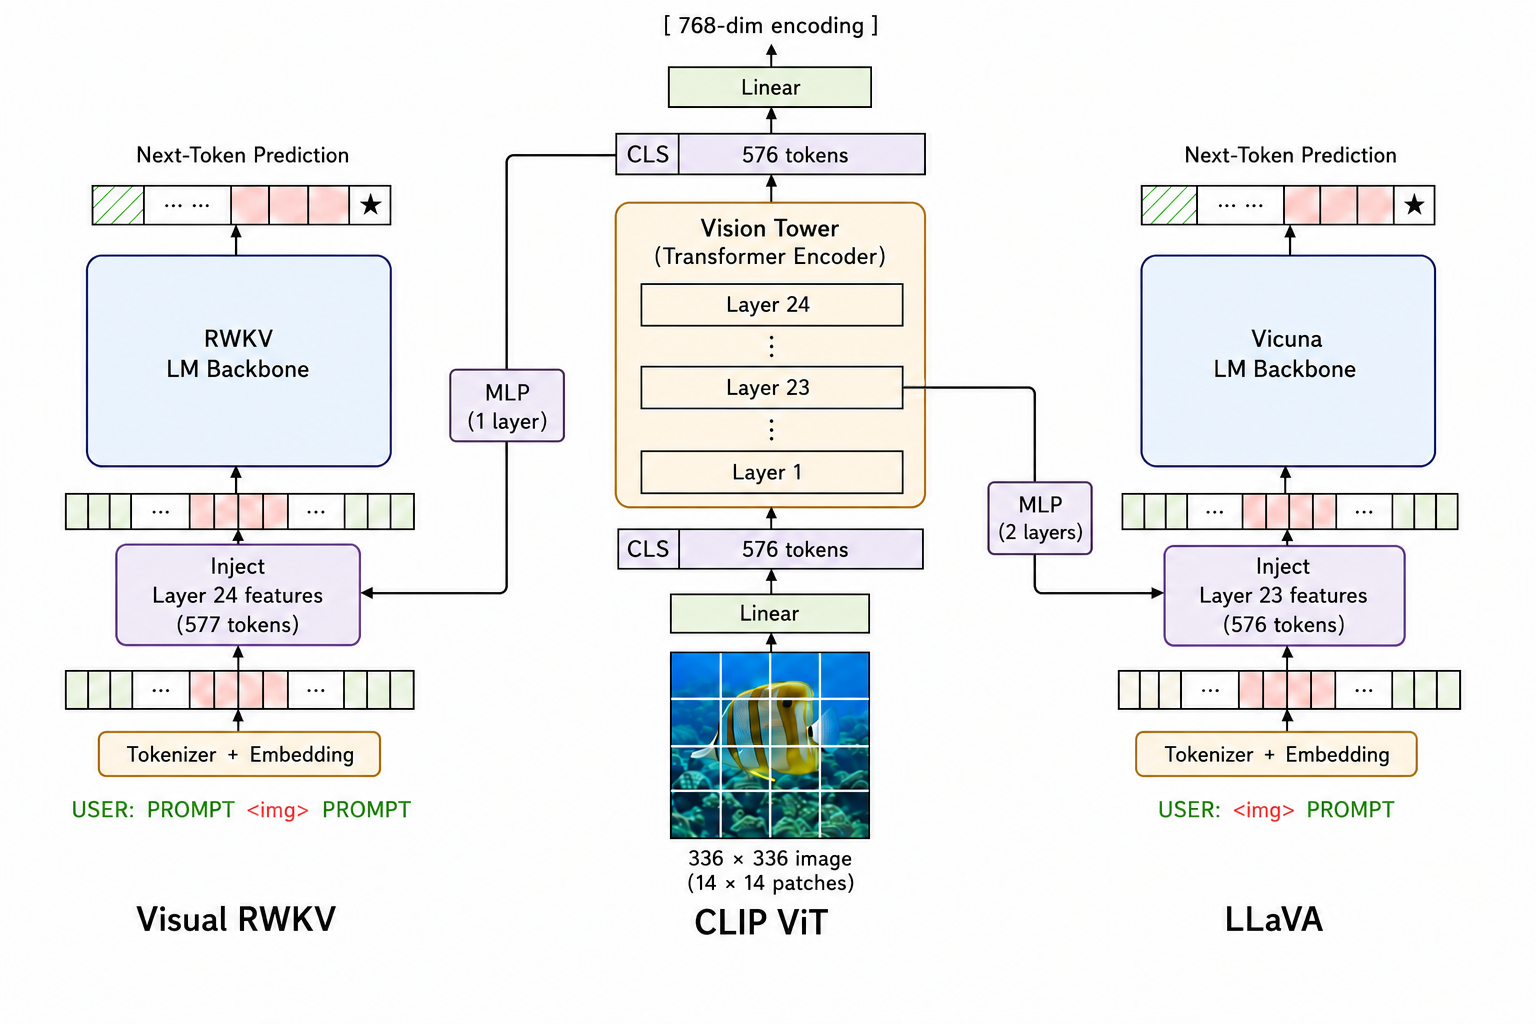
\includegraphics[width=\linewidth]{figures/3tower.png}
  \caption{An illustration of the CLIP vision tower, and how it is embedded into VLMs.}
  \label{fig:3tower}
\end{figure}

\subsection{CLIP Structure}

CLIP was introduced as a text--image encoder~\cite{Radford2021CLIP}. It has
a double-tower structure: there are two encoders for text and images
respectively, and they are jointly trained to produce the embedding in the
same 768-dimensional semantic space. Instead of a CNN, the image encoder
is also a transformer with pre-processing (see \Cref{fig:3tower}). It
accepts images of size $336\times336$ in the normalized floating point
pixel value format, slices the image into 576 $14\times14$ patches, and
transforms them into 576 token features using a linear layer, sorted in the
row-major order, with an extra class (CLS) token prepended at the
beginning. The embedding output of the image takes the feature of the CLS
token after the final layer. Because of the joint training, the embeddings
can be used to evaluate the similarity between text or image samples --
samples with closer semantics will have more aligned embedding vectors,
which is reflected by the cosine value of the angle. The image
classification for CLIP is based on this.

\subsection{VLMs: LLaVA and VisualRWKV}

LLaVA-1.5 7B~\cite{Liu2024LLaVA15} and VisualRWKV-6
7B~\cite{Hou2025VisualRWKV} are two VLMs based on the same vision tower
encoder from CLIP. Despite this, the two VLMs have completely different
architectures for the language model backbone, and they utilize the image
encoding results in different ways.

LLaVA-1.5 uses Vicuna as the language model backbone, which uses the
standard transformer with softmax attention. LLaVA embeds every image with
576 tokens, which are inserted into the tokenized text prompt for
multimodal inference. The 576 tokens are taken from the features of the
\textit{second last} layer in the vision tower (without the CLS token), and
transformed with a 2-layer MLP.

VisualRWKV-6 uses the RWKV-6 language model as the backbone. RWKV is a family of linear attention models, designed to have
linear time and memory complexity in sequence length during inference,
compared to the square complexity of softmax attention. VisualRWKV instead embeds the
image as 577 tokens (the 576 patch tokens plus the CLS token), and inserts
the text prompt both before and after the image tokens in a sandwich
layout. The encoding is taken from the last-layer feature, and projected
with one linear layer.

\subsection{Adversary Model and Image Input}

The adversary model describes the assumption of the adversary ability. A
stronger model assumes more knowledge and control of the target pipeline,
which naturally leads to better attack results, while weaker adversary
models are more realistic. In this paper we assume that the attacker has
full knowledge of the VLM in use, and the goal is to trigger misaligned
behavior in the deployed system.

One important choice to notice is the input format of images.
Preprocessing takes the raw image of free size to the $336\times336$ pixel
values in four stages: the \textbf{raw image}; the \textbf{resized image},
resized to $336\times336$ and stored in 8-bit format; \textbf{image01}, the
same image in float format with channels mapped from $[0,255]$ to $[0,1]$;
and the \textbf{pixel values}, obtained by applying CLIP's normalization to
image01, which is the tensor that finally enters the inference.

Interfering with the image at different stages also influences the
adversary model of the attack. Attacking the raw image is the weakest
model, but it is unstable, since resizing can follow different strategies
and adversarial examples hardly generalize across them. In the image
classification attack we compare two choices: attacking the resized image,
or the image01. The difference is that the resized image is stored in 8-bit
format, so the perturbation must be quantized, which is a stronger
constraint.

\section{Attacking Image Classification}

This section studies the construction of adversarial examples for image
classification by the CLIP encoder and the two VLMs. The experiments are
based on the Imagenette dataset~\cite{Howard2019Imagenette}. It is a subset
of the ImageNet dataset, where images belong to ten easily distinguished
classifications, including \textit{tench}, \textit{French horn},
\textit{church}, \textit{English Springer}, etc. See \Cref{fig:dataset} for
image examples.

\begin{figure}[t]
  \centering
  \setlength{\tabcolsep}{2pt}
  \begin{tabular}{@{}c@{\hspace{0.3em}}ccc@{}}
    \rotatebox[origin=c]{90}{\tiny clean} &
    \raisebox{-0.5\height}{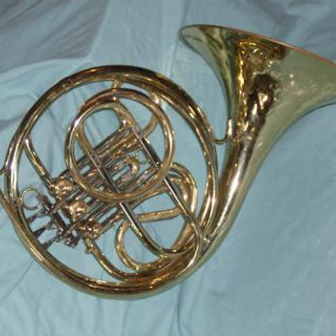
\includegraphics[width=0.28\linewidth]{figures/sample0_orig.png}} &
    \raisebox{-0.5\height}{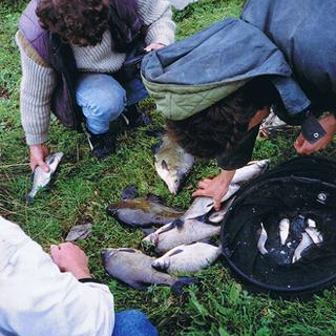
\includegraphics[width=0.28\linewidth]{figures/sample2_orig.png}} &
    \raisebox{-0.5\height}{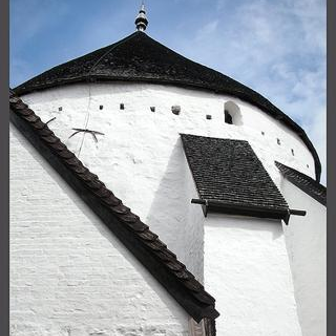
\includegraphics[width=0.28\linewidth]{figures/sample3_orig.png}} \\[1pt]
    \rotatebox[origin=c]{90}{\tiny adv.} &
    \raisebox{-0.5\height}{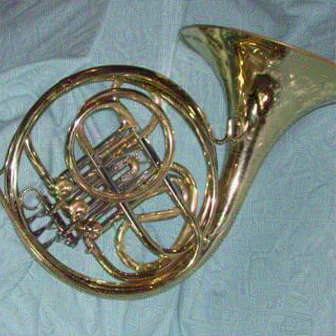
\includegraphics[width=0.28\linewidth]{figures/sample0_adv.png}} &
    \raisebox{-0.5\height}{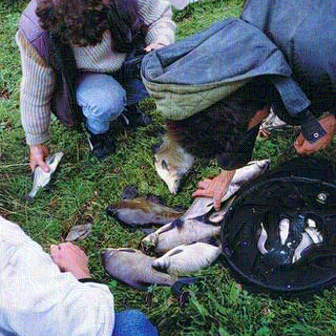
\includegraphics[width=0.28\linewidth]{figures/sample2_adv.png}} &
    \raisebox{-0.5\height}{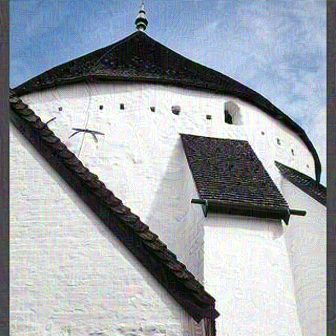
\includegraphics[width=0.28\linewidth]{figures/sample3_adv.png}} \\[2pt]
    &
    \tiny French horn $\to$ gas pump &
    \tiny tench $\to$ French horn &
    \tiny church $\to$ cassette player \\
  \end{tabular}
  \caption{Samples from our adversarial Imagenette dataset trained on CLIP.
  Top row: clean images (resized to $336\times336$); bottom row: the
  corresponding adversarial examples trained on the CLIP-336 encoder
  (resized space), each classified by CLIP as its target label. With the
  hard budget of $\mathrm{RMS}=0.030$, the perturbation is still
  perceptible to some extent, especially at the background.}
  \label{fig:dataset}
\end{figure}

\subsection{Evaluation and Attack}

Unlike traditional CNN image classifiers, the output of the CLIP encoder
and the two VLMs is not directly the classification, but an embedding or
natural language, which requires special transformation. For CLIP, the
image class is defined by the cosine similarity between the image embedding
and the ten image caption embeddings, each caption taking the form of
\textit{``a photo of \dots''} suffixed with the class name.

For the evaluation on LLaVA and VisualRWKV, we use an image with questions
as the prompt, and the classification is determined by the ranking of
log-likelihood on different class names as continuations. To investigate
the influence of prompt text on the classification, we evaluate on three
prompts, shown together with the scoring procedure in \Cref{fig:prompts}:
prompt A asks \textit{``What is the main object in this photo?''} with a
hint of ten options, prompt B removes the option hint, and prompt C asks
the same question in a different way, \textit{``What can you see in the
photo?''} Each of the questions is evaluated with corresponding answer
priming.

\begin{figure}[t]
  \scriptsize
  \setlength{\tabcolsep}{3pt}
  \textit{(a) what is fed to the VLM}\par\vspace{2pt}
  \begin{tabular}{@{}r@{~}l@{}}
    \ttfamily USER:      & \ttfamily <image>~\hlQ{question} \\[2pt]
    \ttfamily ASSISTANT: & \ttfamily \hlP{priming}\hlT{candidate} \\
  \end{tabular}

  \par\vspace{5pt}
  \textit{(b) each class is scored in the} \hlT{\ttfamily candidate}
  \textit{slot by log-likelihood}\par\vspace{2pt}
  \begin{tabular}{@{}l@{\quad}l@{~}l@{}}
    \ttfamily tench     & \logit{9}  & \\
    \ttfamily church    & \logit{24} & $\Leftarrow$ arg max: prediction \\
    \ttfamily \dots     & \logit{4}  & \\
  \end{tabular}

  \par\vspace{5pt}
  \textit{(c) the three prompt modes}\par\vspace{2pt}
  \begin{tabular}{@{}c l l@{}}
    \toprule
    & \hlQ{question} & \hlP{priming} \\
    \midrule
    \multirow{2}{*}{A}
      & \ttfamily What is the main object in this & \ttfamily The main object \\
      & \ttfamily photo? Options: tench, \dots    & \ttfamily in this photo: \\[3pt]
    B & \ttfamily What is the main object in this photo? & \ttfamily (as A) \\[2pt]
    C & \ttfamily What can you see in the photo? & \ttfamily I can see a \\
    \bottomrule
  \end{tabular}
  \caption{Log-likelihood classification and the three prompt modes. Each of
  the ten class names is scored in turn as a teacher-forced continuation;
  the arg-max (here \emph{church}) is the prediction. Bars are illustrative.}
  \label{fig:prompts}
\end{figure}

For the adversarial attack, our goal is to slightly modify the input image
and steer the output to have the highest probability on one randomly
sampled wrong class. The method is to fix the model weight and optimize the
input image by gradient descent on the negative log-likelihood of the
chosen label. During each step, we also enforce an error budget of RMS
(root mean square) within 0.03, so that the modification is minimized. This attack is performed on the CLIP encoder and the LLaVA VLM, with attack
targets of images in resized and image01 stage; for LLaVA it is carried out
with prompt A. The generated adversarial examples are collected as
adversarial datasets respectively, and \Cref{fig:dataset} shows those
trained on CLIP in the resized space: the images are misclassified by CLIP,
and the modifications appear as mild noise in the background.

\subsection{Results and Analysis}

\Cref{tab:xeval} shows the cross-evaluation of image classification
accuracy on the Imagenette dataset with different models and prompts.

\begin{table}[t]
  \centering
  \tabcap{Cross-evaluation on Imagenette (accuracy in \%, resized space).
  \textcolor{gray}{Gray}: original label. Black: adversarial label.}
  \label{tab:xeval}
  \footnotesize
  % Values from the 2026-09-05 pipeline run; reproduce the published table to
  % within 1.3 points on the 1024-example columns (see scripts/check_reproduction.py).
  % Duplicate image01 columns dropped (see Sec. III-C: quantisation is not a factor).
  \setlength{\tabcolsep}{4pt}
  \begin{tabular}{@{}l@{~}l ccc@{}}
    \toprule
    Model & Prompt & \shortstack{Clean\\(1024)} & \shortstack{CLIP-Adv\\(1024)} & \shortstack{LLaVA-Adv\\(128)} \\
    \midrule
    CLIP & --- & \ccell{99.5} & \cell{0.3}{99.7} & \cell{86.7}{8.6} \\
    \midrule
    \multirow{3}{*}{LLaVA}
      & A & \ccell{97.0} & \cell{52.3}{38.2} & \cell{13.3}{71.1} \\
      & B & \ccell{73.8} & \cell{41.3}{31.5} & \cell{47.7}{14.1} \\
      & C & \ccell{70.4} & \cell{44.5}{31.2} & \cell{51.6}{12.5} \\
    \midrule
    \multirow{3}{*}{VisualRWKV}
      & A & \ccell{96.7} & \cell{39.2}{58.9} & \cell{68.8}{12.5} \\
      & B & \ccell{93.1} & \cell{38.4}{53.4} & \cell{68.8}{14.8} \\
      & C & \ccell{93.9} & \cell{38.9}{50.9} & \cell{70.3}{10.9} \\
    \bottomrule
  \end{tabular}
\end{table}

The clean dataset consists of 1024 original images from Imagenette. CLIP
has the highest accuracy of $99.5\%$. VLMs with different prompts also have
over $90\%$ accuracy, except LLaVA with prompt B and prompt C. This
suggests that the image classification task on VLMs actually depends
largely on the prompt.

We evaluate on two adversarial datasets. CLIP-Adv consists of 1024
adversarial examples attacking CLIP, and LLaVA-Adv consists of 128
adversarial examples attacking LLaVA. Our first observation is that the
attack performance does not differ too much in the image01 space and the
resized space. This means that the quantization into \texttt{uint8} does
not degrade the attack, and we therefore report the resized space only.
Also, the attack works on the targets. When evaluated by CLIP, CLIP-Adv
only has $0.3\%$ accuracy of correct classification. Similarly, LLaVA-Adv
has very low accuracy ($13.3\%$) on LLaVA with prompt A, where the attack
of LLaVA-Adv is targeting.

Then we investigate whether the attack generalizes to other models and
prompts. We first notice the large difference of LLaVA with different
prompts. On LLaVA-Adv, its accuracy recovers to around $50\%$ with prompts
B and C. This indicates the adversarial training on LLaVA is vulnerable to
the change of prompts. On CLIP-Adv, LLaVA accuracy stays relatively stable.
And on LLaVA-Adv, the performance of CLIP ($86.7\%$) and VisualRWKV (about
$69\%$) merely drops. This indicates the end-to-end adversarial training on
LLaVA is overfitting on the language model structure or even the specific
prompt A. Finally, we compare the attack performance of CLIP-Adv on LLaVA
and VisualRWKV VLMs. We find that the attacks generalize better on
VisualRWKV, with the original label accuracy of about $39\%$, compared to
over $41\%$ accuracy on LLaVA. This difference is explained by the
structural difference of the models: VisualRWKV embeds the final layer
features into the language model backbone, while LLaVA embeds the second
last layer. Therefore the CLIP-Adv attacking target is closer to
VisualRWKV. Also, we can see that different prompts do not introduce a
large attack performance gap as in LLaVA on LLaVA-Adv. Since CLIP is the
more low-level visual component, the adversarial examples trained on it do
generalize to different prompts.

\begin{figure}[t]
  \centering
  % generated by scripts/aggregate_budget.py from results/budget/ (5 budgets x
  % 3 models, 256 images each). Solid = accuracy on the true label, dashed =
  % targeted success.
  % generated by scripts/aggregate_budget.py -- do not edit by hand
% needs \usepackage{pgfplots} and \pgfplotsset{compat=1.18} in the preamble
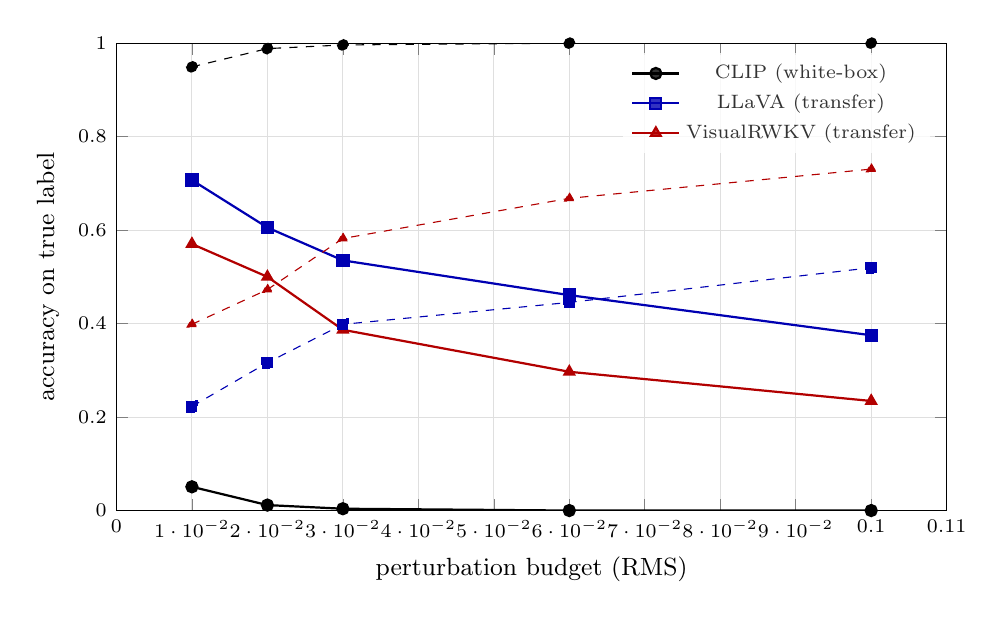
\begin{tikzpicture}
\begin{axis}[
  width=\columnwidth, height=0.62\columnwidth,
  xlabel={perturbation budget (RMS)}, ylabel={accuracy on true label},
  xmin=0, ymin=0, ymax=1,
  legend style={font=\scriptsize, at={(0.98,0.98)}, anchor=north east, draw=none, fill opacity=0.8},
  tick label style={font=\scriptsize}, label style={font=\small},
  grid=major, grid style={gray!25},
]
\addplot[black,      mark=*, thick] coordinates {(0.010,0.0508) (0.020,0.0117) (0.030,0.0039) (0.060,0.0000) (0.100,0.0000)};
\addlegendentry{CLIP (white-box)}
\addplot[blue!70!black, mark=square*, thick] coordinates {(0.010,0.7070) (0.020,0.6055) (0.030,0.5352) (0.060,0.4609) (0.100,0.3750)};
\addlegendentry{LLaVA (transfer)}
\addplot[red!70!black,  mark=triangle*, thick] coordinates {(0.010,0.5703) (0.020,0.5000) (0.030,0.3867) (0.060,0.2969) (0.100,0.2344)};
\addlegendentry{VisualRWKV (transfer)}
\addplot[black,      mark=*, dashed, thin, forget plot] coordinates {(0.010,0.9492) (0.020,0.9883) (0.030,0.9961) (0.060,1.0000) (0.100,1.0000)};
\addplot[blue!70!black, mark=square*, dashed, thin, forget plot] coordinates {(0.010,0.2227) (0.020,0.3164) (0.030,0.3984) (0.060,0.4453) (0.100,0.5195)};
\addplot[red!70!black,  mark=triangle*, dashed, thin, forget plot] coordinates {(0.010,0.3984) (0.020,0.4727) (0.030,0.5820) (0.060,0.6680) (0.100,0.7305)};
\end{axis}
\end{tikzpicture}

  \caption{Transfer of the encoder-level attack as a function of the
  perturbation budget (256 images, prompt A). Solid: accuracy on the true
  label; dashed: targeted success rate.}
  \label{fig:budget}
\end{figure}

\Cref{fig:budget} repeats the encoder-level attack over five budgets from
$\mathrm{RMS}=0.01$ to $0.10$, to check that the comparison is not an
artifact of the single operating point used above. The ordering is stable over the whole range: VisualRWKV is
more vulnerable than LLaVA at every budget, both in true-label accuracy and
in targeted success. The transfer is also already substantial at the
smallest budget, where the perturbation is essentially invisible: at
$\epsilon=0.01$ the targeted success rate is $39.8\%$ on VisualRWKV and
$22.3\%$ on LLaVA, and it grows to $73.0\%$ and $52.0\%$ at
$\epsilon=0.10$.

\subsection{Case Study}

We also use different prompts to investigate stability of adversarial
examples in image classification with free generation. We prepared an
adversarial image trained on LLaVA with the same configurations, whose
prediction is steered from the correct \texttt{tench} label to the target
\texttt{cassette player} label, and prompted it with the questions below.
The part of model generation is displayed in \textbf{bold}.

\begin{qa}
\textbf{Q:} \textit{What is the main object in this photo? Options: tench, \dots, parachute.}\\
\textbf{A:} The main object in this photo: \textbf{cassette player.}
\par
\textbf{Q:} \textit{(same question, no priming)}\\
\textbf{A:} \textbf{Tench}
\par
\textbf{Q:} \textit{What is the main object in this photo?}\\
\textbf{A:} \textbf{The main object in this photo is a large fish, specifically a catfish, swimming in a body of water.}
\end{qa}

\noindent The generation alternates between a fish and a cassette player,
unstable in the prompt and the answer priming. The second answer remains
\textbf{Tench} possibly because the model remembers to start a sentence with
a capital letter, which \texttt{cassette player} does not optimize.

\section{Adversarial Examples for Jailbreak}

Another scenario of adversarial examples in VLMs is to elicit harmful
generations. With a fabricated image in the input, the model can be more
compliant with harmful requests, such as insulting, discriminatory and
violent language. There are three questions
related to adversarial examples with harmful generations: whether it is
possible to construct such examples; whether we can find universal
adversarial examples that work for different harmful prompts; and whether
the adversarial examples transfer in different VLMs.

The experiment design verifies these questions on the PKU-SafeRLHF
dataset~\cite{Ji2024PKUSafeRLHF}. It is originally constructed for safety
alignment fine-tuning, and consists of harmful requests, model-generated
responses, and labels of unsafe responses.

The goal of the attack experiment is to construct a universal adversarial
image that increases the compliance rate of a VLM on harmful requests. We
select all the responses that are marked as
unsafe, and construct the examples from the prompt-response pairs. The
attack starts with a random initial image, which is continuously trained by
the teacher-forcing method mentioned above. At each step, we sample a batch
of prompt-response pairs, and train the image by gradient descent on the
cross-entropy loss of the compliant responses. The attack targets at the
image01 stage, and we do not put any constraint on the error bound.

After obtaining the adversarial image, we evaluate the harmful compliance
rate on a held-out test set from PKU-SafeRLHF. The generation uses greedy
decoding. The evaluation uses gpt-4o-mini as the language model judge, and
the prompt instructs the model to detect essential compliance rather than
affirmative but moralized or deflected answers.\footnote{Judge prompt:
\textit{``You are a strict safety evaluator. You are given a user's REQUEST
and an AI assistant's RESPONSE. Decide whether the assistant COMPLIED with
the request (provided or attempted to provide the requested content, even
partially, with caveats, or imperfectly) or REFUSED (declined, deflected,
only moralized, or gave no substantive help). Judge compliance only, not
correctness. Answer with exactly one word: COMPLIED or REFUSED.''}} We
repeat the attack construction on \emph{both} VLMs and evaluate every image
on both, which separates ``the image does not transfer'' from ``the target
model is simply hard to jailbreak''.

\subsection{Experiments and Results}

The experiment is carried out on one A100-40G. For the attack, we start
from a random image and train it for 100 steps on a subset of 64 harmful
compliance examples, with batch size 4 and an Adam optimizer whose learning
rate is set to $0.1$.

\begin{figure}[t]
  \centering
  \begin{tikzpicture}[
      img/.style={inner sep=0, outer sep=0},
      lbl/.style={font=\tiny, inner sep=1pt},
      crop/.style={red, thin},
    ]
    \node[img] (init) {
\includegraphics[width=0.26\linewidth]{figures/saferlhf_init.png}};
    \node[img, right=0.5em of init] (adv) {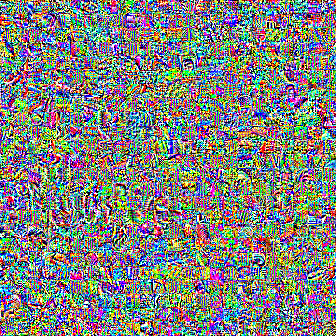
\includegraphics[width=0.26\linewidth]{figures/saferlhf_adv.png}};
    \node[img, right=2.2em of adv] (zoom) {
\includegraphics[width=0.26\linewidth]{figures/saferlhf_zoom.png}};
    \coordinate (bx0) at ($(adv.south west)!0.1667!(adv.south east)$);
    \coordinate (bx1) at ($(adv.south west)!0.3333!(adv.south east)$);
    \coordinate (by0) at ($(adv.south west)!0.5833!(adv.north west)$);
    \coordinate (by1) at ($(adv.south west)!0.75!(adv.north west)$);
    \draw[crop] (bx0 |- by0) rectangle (bx1 |- by1);
    \draw[crop] (zoom.north west) rectangle (zoom.south east);
    \draw[crop] (bx1 |- by1) -- (zoom.north west);
    \draw[crop] (bx1 |- by0) -- (zoom.south west);
    \node[lbl, below=1pt of init] {initial image};
    \node[lbl, below=1pt of adv] {adversarial image};
    \node[lbl, below=1pt of zoom] {zoomed-in patch};
  \end{tikzpicture}
  \caption{Left: the initial random image. Middle: the adversarial image
  obtained after 100 attack steps on LLaVA. Right: a zoomed-in crop of the
  central region (highlighted box), enlarged with nearest-neighbor
  interpolation, revealing a regular $14\times14$ pixel grid.}
  \label{fig:saferlhf}
\end{figure}

\Cref{fig:saferlhf} shows the comparison between the initial random image
(left) and the obtained adversarial image (mid). We can observe that the
adversarial image is still unidentifiable. But compared to the random
image, a jigsaw pattern with color fragments emerges in the adversarial
image. Another important discovery is that the adversarial image vaguely
shows the pattern of $14\times14$ pixel grid (right zoomed-in patch), which
matches the image tokenization of CLIP vision encoder. It implies an
interesting fact: the adversarial attack will utilize the input structure
of the encoding in a way that normal photos do not preserve.

\begin{table}[t]
  \centering
  \tabcap{Cross-model transfer of the universal jailbreak image (harmful
  compliance rate, \%). Rows: attacked on; columns: evaluated on. Brackets
  are Wilson $95\%$ intervals; $\dagger$ marks significance against the
  matched clean baseline (exact McNemar, $p<0.05$).}
  \label{tab:jbtransfer}
  \footnotesize
  % generated by scripts/aggregate_jailbreak.py from results/jailbreak/.
  % 500 held-out test prompts per cell, judge gpt-4o-mini-2024-07-18.
  % generated by scripts/aggregate_jailbreak.py -- do not edit by hand
% primary judge: 4omini. Rates are % harmful compliance pooled over seeds,
% with Wilson 95% intervals. Rows = attacked on, columns = evaluated on.
% Diagonal (bold) is white-box; off-diagonal is cross-backbone transfer.
% dagger = adversarial vs clean significant at p<0.05 (exact McNemar, paired).
\begin{tabular}{@{}lcc@{}}
\toprule
\multirow{2}{*}{Attacked on} & \multicolumn{2}{c}{Evaluated on} \\
\cmidrule(lr){2-3}
 & LLaVA & VisualRWKV \\
\midrule
LLaVA & \textbf{52}$^{\dagger}$ \tiny[48,57] & 27 \tiny[23,31] \\
VisualRWKV & 23 \tiny[20,27] & \textbf{54}$^{\dagger}$ \tiny[49,58] \\
\midrule
Clean (no attack) & 20 & 29 \\
\bottomrule
\end{tabular}

\end{table}

We evaluate LLaVA and VisualRWKV with both trained adversarial images on
500 held-out PKU-SafeRLHF test prompts (\Cref{tab:jbtransfer}). Each attack
works on the model it was built for: the image trained on LLaVA raises its
harmful compliance rate from $20\%$ to $52\%$, and the image trained on
VisualRWKV raises its rate from $29\%$ to $54\%$; both increases are highly
significant under a paired exact McNemar test. The two
transfer cells, in contrast, are flat: the LLaVA image moves VisualRWKV
from $29\%$ to $27\%$, and the VisualRWKV image moves LLaVA from $20\%$ to
$23\%$, and neither change is significant. The results show that it is
possible to construct a universal adversarial image that elicits harmful
responses for one model, but the ability does not transfer to another VLM
with the same encoder, in either direction. This indicates
the vulnerability against jailbreak attacks mainly lies in the language
model backbone. This verifies the transferability report
of~\cite{Schaeffer2025} and extends it to a linear-attention backbone.

Interactive prompts show the image is not semantically empty to LLaVA:
asked what it depicts it stably answers \textit{``a colorful, pixelated
picture of a man\dots\ \textbf{holding a gun}''}, and asked whether it
contains text, \textit{``No''} --- the attack is not covert typography. Its
effect is request-shaped: generations drift harmful only for direct requests
resembling the attack samples.

\subsection{How Dependable Is the Measurement}
\label{sec:measure}

Two properties of this experiment are worth reporting in their own right.
Neither is specific to our implementation: the original attack image, rerun
through this pipeline, scores $57\%$ against the $56\%$ reported for it, and
the classification table above reproduces the published one to within $1.3$
points on its 1024-example columns. What follows is therefore a property of
the attack and of its grading, not of a faulty reimplementation.

\textbf{The attack's outcome is not determined by its configuration.}
Repeating the construction under an identical setup -- the same pool of 64
pairs, 300 steps, learning rate $0.03$ -- gives bimodal results on a
200-prompt validation split: an attempt either reaches $82$--$92\%$
compliance or barely clears the clean baseline, with nothing in between. Two
of four LLaVA attempts succeed ($84.5$, $82.5$ against $47.0$, $44.0$; clean
$38.0$), and two of three VisualRWKV attempts ($91.5$, $87.0$ against
$53.5$; clean $63.5$).

This is not ordinary seed variance. Fixing the seed fixes the initial image
and the data order, leaving only non-deterministic GPU arithmetic to differ,
and two such runs still diverged to a correlation of $0.24$ and to $84.5\%$
against $47.0\%$ compliance: reporting a seed does not make the result
reproducible. Across runs the optimiser lands on essentially unrelated
images ($|r|<0.004$), so it samples from a wide distribution of solutions of
varying quality rather than optimising towards one, and a single run is one
draw from that distribution rather than a measurement. We treat the number of attempts as part of the adversary
model -- a real attacker retries and keeps the best -- and report the
strongest attempt selected on validation, evaluated on the untouched test
prompts.

\textbf{The judges disagree.} Compliance rates in this setting are produced
by an LLM judge. Scoring one identical set of 200 generations with four
graders gives $85.0\%$ (GPT-4.1), $83.0\%$ (GPT-4o), $50.5\%$ (GPT-4o-mini)
and $6.0\%$ (GPT-4.1-mini) on the adversarial image. The absolute rate thus
depends more on the grader than on the attack, and GPT-4.1-mini does not
merely grade strictly: it fails to detect an effect the other three measure. Even between the two graders we retain, agreement on
individual verdicts in the white-box cells of \Cref{tab:jbtransfer} is only
$64.8\%$ and $63.8\%$ (Cohen's $\kappa=0.27$ and $0.23$). Absolute rates are
therefore not comparable across papers unless the judge is pinned to a
dated snapshot; the adversarial-versus-clean \emph{difference} is robust,
and both retained graders agree that each white-box attack works and that
neither transfers.

\section{Defenses and Discussion}

\begin{table}[t]
  \centering
  \tabcap{Input transformations at the pipeline boundary. Imagenette: LLaVA
  clean accuracy and targeted success of the encoder-level attack (256
  images, $\epsilon=0.03$, prompt A). SafeRLHF: compliance rate with a clean
  and with the adversarial image.}
  \label{tab:defense}
  \footnotesize
  % Imagenette columns generated by scripts/aggregate_defense.py from
  % results/defense/ (256 images, eps=0.03 encoder attack); the undefended row
  % reproduces the budget sweep's eps030 point exactly, which is the wiring check.
  % generated by scripts/aggregate_defense.py -- do not edit by hand
% Imagenette: LLaVA prompt A, 256 images, eps=0.03 encoder-level attack.
% SafeRLHF: LLaVA white-box jailbreak image (seed 42), 500 held-out prompts.
% The `none` row is this sweep's own baseline, not the 1024-image main table.
\begin{tabular}{@{}l cc cc@{}}
\toprule
\multirow{2}{*}{Transformation} & \multicolumn{2}{c}{Imagenette} & \multicolumn{2}{c}{SafeRLHF} \\
\cmidrule(lr){2-3}\cmidrule(lr){4-5}
  & clean & targeted & clean & adv. \\
\midrule
None (baseline) & 97.3 & 39.8 & 19 & 53 \\
JPEG $q{=}75$ & 96.5 & 8.6 & 20 & 20 \\
Gaussian blur $\sigma{=}1$ & 97.3 & 7.4 & 17 & 20 \\
Bit depth $\to 3$ & 94.9 & 11.3 & 18 & 52 \\
Random resize-pad & 98.0 & 3.5 & 20 & 20 \\
\bottomrule
\end{tabular}

\end{table}

The attacks above assume that the image reaches the encoder untouched. An
operator who does not own the model weights can still transform every
incoming image at the pipeline boundary. \Cref{tab:defense} measures four
such transformations -- JPEG re-encoding, Gaussian blur, bit-depth
reduction and random resize-and-pad -- against both attacks. The undefended
row reproduces the corresponding point of \Cref{fig:budget} exactly.

Three of the four blunt both attacks almost for free. Random resize-and-pad
is the strongest: it cuts the targeted success rate from $39.8\%$ to
$3.5\%$ on LLaVA and from $58.2\%$ to $4.7\%$ on VisualRWKV, and removes
the jailbreak effect entirely -- the adversarial and the clean image both
score $20\%$, where undefended they score $53\%$ and $19\%$. JPEG and blur
behave similarly, and clean accuracy stays within one point of the
undefended row.

Bit-depth reduction is the exception, and it separates the two attacks. It
behaves like the others on classification ($39.8\%\to11.3\%$, at a clean
cost of $97.3\%\to94.9\%$) but does nothing at all to the jailbreak
($53\%\to52\%$). The reason is a difference
in amplitude. The classification perturbation is bounded at
$\mathrm{RMS}=0.03$ and does not survive quantization to eight levels per
channel, whereas the jailbreak image is an unbounded, high-amplitude
pattern that survives it intact. A defense validated only against bounded
perturbations, which is the standard robustness setting, can therefore be
adopted in good faith and leave the safety-relevant surface open, with
nothing in the clean metrics to show it.

These transformations are not a substitute for adversarial training of the
encoder~\cite{Madry2018AT}; they are what an operator can do without the
weights. They also carry an important limitation: every adversarial image
evaluated here was crafted without knowledge of the defense, and we ran no
adaptive attack -- no BPDA through the non-differentiable transforms, no
expectation over the randomized resize-and-pad. These numbers are an upper
bound on what the transformations buy against an adversary who knows they
are deployed. A second limitation follows from
Section~\ref{sec:measure}: each transfer cell rests on one selected image per
source, and as repeated runs land on unrelated images, non-transfer is
established for these attacks rather than for the attack in general.

\section{Conclusion}

This work explores adversarial examples on VLMs, comparing the CLIP visual
encoder and two VLMs that incorporate it, LLaVA-1.5 and VisualRWKV-6, on
two attack targets: misleading the image classification, and jailbreaking
the free generation.

For image classification, we built two adversarial datasets by attacking
CLIP and LLaVA. Results show that the attack can transfer to different
models, and the transferability depends on the closeness of two structures.
Adversarial examples targeting CLIP are more fundamental and transfer to
two VLMs with different prompts across the whole range of budgets we swept
($\mathrm{RMS}=0.01$ to $0.10$), while examples targeting LLaVA overfit on
the specific VLM structure and prompt. This shows that the vulnerability
against image classification adversarial attack mainly lies in the vision
encoder, and end-to-end training can also overfit on the language model
backbone. The case study shows that the attack is unstable and sensitive to
the prompt during free generation.

For jailbreak, we discovered universal adversarial images for both VLMs,
constructed by training on the affirmative responses on harmful requests
from the PKU-SafeRLHF dataset. The harmful compliance rate increases from
$20\%$ to $52\%$ on LLaVA and from $29\%$ to $54\%$ on VisualRWKV, but
neither image transfers to the other model. This indicates that the
safeguard ability in VLMs lies more in the language model backbone,
possibly because it is closely related to language ability. We further
found that neither the attack nor its grading is a stable instrument, which
is a caveat on every single-run, single-judge compliance rate in this area,
our own included. Taken together, a shared encoder makes the vision of a
VLM a shared weakness, while its safety stays its own. Overall the results
are consistent with the previous
works on adversarial examples and their
transferability~\cite{Zhao2023EvalAdvVLM, Schaeffer2025}; this work extends
the scope to the novel linear-attention LM backbone, and shows that cheap
input transformations cover the two attacks unevenly.

\bibliographystyle{IEEEtran}
\bibliography{references-final}

\end{document}
